\documentclass[pdf]{beamer}
\mode<presentation>
{
	\usetheme{Warsaw}
}
\usepackage[utf8]{inputenc}
\usepackage[portuguese]{babel}
\usepackage[T1]{fontenc}
\usepackage{amsmath}
\usepackage{amsfonts}
\usepackage{amssymb}
\usepackage{makeidx}
\usepackage{graphicx}
\usepackage{hyperref}
\author{Welson Jr}
\title{Codificação Radix-64/base64: exemplos, pontos fortes e fracos}
\subtitle{IA012 - 2013}
\makeindex
\begin{document}
\begin{frame}
\transdissolve
\maketitle
\end{frame}
\section{Agenda}
\begin{frame}{Agenda}
\transdissolve
	\tableofcontents
\end{frame}

\AtBeginSection[]
{
\begin{frame}
	\tableofcontents[currentsection]
\end{frame}
}

\section{O que é Base 64}
\subsection{Introdução}
\begin{frame}{Introdução}
\transdissolve
Base ou Radix 64 é uma técnica que converte uma entrada de dados binários em texto de caracteres imprimíveis para que possam ser transportados por qualquer meio de transmissão.
\pause
\begin{block}{De acordo com a RFC 3548}
Base encoding of data is used in many situations to store or transfer data in environments that, perhaps for legacy reasons, are restricted to US-ASCII data.  Base encoding can also be used in new applications that do not have legacy restrictions, simply because it makes it possible to manipulate objects with text editors.
\end{block}
\end{frame}
\subsection{Funcionamento}
\begin{frame}{Funcionamento}
\transdissolve
\begin{figure}[ht]
\begin{center}
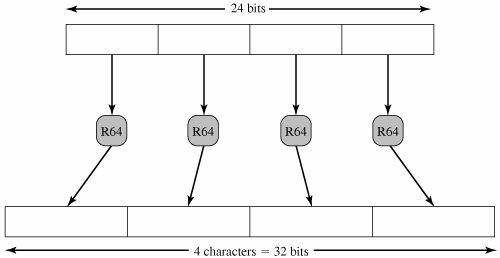
\includegraphics[width=1\textwidth]{radix64.jpg}
\end{center}
\end{figure}
\end{frame}
\begin{frame}{Funcionamento}
\begin{itemize}
\item A entrada binaria é processada em blocos de 3 octetos, ou 24 bits.\\
\item Cada conjunto de 6 do bloco de 24 bits é mapeado para um carácter Base64.\\
\pause
\item E caso o numero de bytes de entrada não seja divisível por 3?\\
\pause
\begin{enumerate}[{Caso} 1]
\item Falte 1 octeto
\pause
\item Faltem 2 octetos
\end{enumerate}
\end{itemize}
\end{frame}
\subsection{Funcionamento}
\begin{frame}{Funcionamento}
Caso o numero de bytes de entrada não seja divisível por 3, tomam-se as seguintes medidas:
\begin{itemize}
\item Preenche-se com zeros os octetos faltantes, e converte-se normalmente segundo a tabela.
\item Caso falte um octeto, adiciona-se um "=" ao final da sequencia.
\item Caso falte 2 octetos, adiciona-se "==" ao final da sequencia.
\end{itemize}
\end{frame}
\subsection{Caracteres Base 64}
\begin{frame}{Caracteres Base 64}
\transdissolve
\begin{table}
\scalebox{0.70}{
\begin{tabular}{||c|c|c|c|c|c|c|c||}
\hline
\textbf{Valor} & \textbf{Char} & \textbf{Valor} & \textbf{Char} & \textbf{Valor} & \textbf{Char} & \textbf{Valor} & \textbf{Char} \\ 
\hline \hline
0 & A & 16 & Q & 32 & g & 48 & w \\
1 & B & 17 & R & 33 & h & 49 & x \\
2 & C & 18 & S & 34 & i & 50 & y \\
3 & D & 19 & T & 35 & j & 51 & z \\
4 & E & 20 & U & 36 & k & 52 & 0 \\
5 & F & 21 & V & 37 & l & 53 & 1 \\
6 & G & 22 & W & 38 & m & 54 & 2 \\
7 & H & 23 & X & 39 & n & 55 & 3 \\
8 & I & 24 & Y & 40 & o & 56 & 4 \\
9 & J & 25 & Z & 41 & p & 57 & 5 \\
10 & K & 26 & a & 42 & q & 58 & 6 \\
11 & L & 27 & b & 43 & r & 59 & 7 \\
12 & M & 28 & c & 44 & s & 60 & 8 \\
13 & N & 29 & d & 45 & t & 61 & 9 \\
14 & O & 30 & e & 46 & u & 62 & + \\
15 & P & 31 & f & 47 & v & 63 & / \\ 
& & & & & & (pad) & = \\
\hline
\end{tabular}}
\caption{Tabela de codificaçao}\label{tab:table_cod}
\end{table}
\end{frame}
\transdissolve
\section{Exemplos de transformação}
\subsection{Exemplo 1}
\begin{frame}{Exemplo 1}
\transdissolve
\begin{table}
\begin{center}
\scalebox{0.65}{
\begin{tabular}{|c|cccccc|cccccc|cccccc|cccccc|}\hline
\textbf{Texto} & \multicolumn{8}{c|}{M} &\multicolumn{8}{c|}{a} &\multicolumn{8}{c|}{n} \\ \hline
\textbf{ASCII} & \multicolumn{8}{c|}{77} & \multicolumn{8}{c|}{97} & \multicolumn{8}{c|}{110} \\ \hline
\textbf{Binario} & 0 & 1 & 0 & 0 & 1 & 1 & 0 & 1 & 0 & 1 & 1 & 0 & 0 & 0 & 0 & 1 & 0 & 1 & 1 & 0 & 1 & 1 & 1 & 0 \\ \hline
\textbf{Decimal} & \multicolumn{6}{c|}{19} & \multicolumn{6}{c|}{22} & \multicolumn{6}{c|}{5} & \multicolumn{6}{c|}{46} \\ \hline
\textbf{Base64} & \multicolumn{6}{c|}{T} & \multicolumn{6}{c|}{W} & \multicolumn{6}{c|}{F} & \multicolumn{6}{c|}{u} \\
\hline
\end{tabular}}
\end{center}
\end{table}
\end{frame}
\subsection{Exemplo 2}
\begin{frame}{Exemplo 2}
\transdissolve
\begin{table}
\begin{center}
\begin{tabular}{|cc|} \hline
\multicolumn{2}{|c|}{\textbf{Dados de entrada}} \\ \hline
Binário & 00100011 01011100 10010001 \\ \hline
Hexadecimal & 235C91 \\ \hline \hline
\multicolumn{2}{|c|}{\textbf{Codificação Base64}} \\ \hline \hline
Base64 & I1yR \\ \hline
ASCII Bin. & 01001001 00110001 01111001 01010010 \\ \hline
Hexadecimal & 49317952 \\ \hline
\end{tabular}
\end{center}
\end{table}
\end{frame}
\subsection{Exemplo 3}
\begin{frame}{Exemplo 3}
\transdissolve
\begin{table}
\begin{center}
\scalebox{1}{
\begin{tabular}{|c|c|} \hline
\textbf{Texto} & \textbf{Base64 Encoding} \\ \hline \hline
Testando o encoding :) & VGVzdGFuZG8gbyBlbmNvZGluZw== \\ \hline
Testando o encoding : & VGVzdGFuZG8gbyBlbmNvZGluZyA6 \\ \hline
Testando o encoding & VGVzdGFuZG8gbyBlbmNvZGluZyA6 \\ \hline
\end{tabular}}
\end{center}
\end{table}
\end{frame}
\section{Pontos fortes}
\begin{frame}{Pontos fortes}
\transdissolve
\begin{itemize}
\item Faz uso apenas de caracteres universalmente empregados em todos os lugares.
\item Devido a não ter caracteres de controle, essa transformação torna os dados praticamente invulneráveis ao processamento de programas de transporte.
\end{itemize}
\end{frame}
\section{Pontos fracos}
\begin{frame}{Pontos fracos}
\transdissolve
\begin{itemize}
\item Aumenta o tamanho da mensagem em cerca de 33\%. \\
Este overhead pode ser estimado em: $4 \times \lceil \frac{n}{3} \rceil$ bytes para cada byte $n$ de entrada
\item Torna difícil a detecção de SPAM em correio eletrônico.
\end{itemize}
\end{frame}
\section{Usos mais comuns}
\begin{frame}{Usos mais comuns}
\transdissolve
\begin{itemize}
\item PGP
\item MIME
\item S/MIME
\end{itemize}
\end{frame}
\section{Questões}
\begin{frame}{Questões}
\transdissolve
\begin{enumerate}
\item Codifique "123" de ASCII para base 64.
\item É seguro utilizar Base64 como um meio de se proteger uma aplicação de login?
\item Como codificar um dado que possui menos de 6 bits?
\end{enumerate}
\end{frame}
\section{Referencias}
\begin{frame}{Referencias}
\begin{itemize}
\item Stallings, William, \emph{ Criptography and Network Security}, Pearson Prentice Hall, 2008.
\item RFC 3548, The Base16, Base32, and Base64 Data Encodings, \url{http://tools.ietf.org/html}
\item RFC 4648, The Base16, Base32, and Base64 Data Encodings, \url{http://tools.ietf.org/html/rfc4648}
\item Wikipedia, Base64, disponível em: \url{http://en.wikipedia.org/wiki/Base64}
\end{itemize}
\end{frame}
\end{document}
